% =====================================================================
%  Autoresearch Loops: A Causal Study of the Instruction File
%  Thesis defence, 15 minutes, 15 frames.
%  Build:  pdflatex presentation.tex   (run twice for the frame counter)
% =====================================================================
\documentclass[aspectratio=169,11pt]{beamer}

\usetheme{Boadilla}
\usecolortheme{dolphin}
\setbeamertemplate{navigation symbols}{}
\setbeamertemplate{caption}[numbered]
\setbeamercovered{transparent}

\usepackage[T1]{fontenc}
\usepackage{lmodern}
\usepackage{graphicx}
\usepackage{booktabs}
\usepackage{tikz}
\usepackage{pgfplots}
\usepgfplotslibrary{groupplots}
\pgfplotsset{compat=1.18}
\usetikzlibrary{shapes.geometric,arrows.meta,positioning}

\definecolor{accent}{HTML}{B35C1E}
\definecolor{muted}{HTML}{6E6E6E}

\title[Autoresearch Loops]{Autoresearch Loops}
\subtitle{A Causal Study of the Instruction File}
\author[C.\ Block]{Christian Block}
\institute[]{Research project with Prof.\ Ramesh}
\date{\today}                     % <-- replace with the defence date

\begin{document}

\begin{frame}[plain]
  \titlepage
\end{frame}

% ============================================ MOTIVATION & BACKGROUND
\begin{frame}{Manual ML research does not scale}
  \begin{itemize}
    \item Tuning is search, run by hand
    \item One person, one experiment
    \item Overnight budgets sit unused
    \item March 2026: \texttt{autoresearch} automates it
    \item Forked over thirteen thousand times
  \end{itemize}
  \vfill
  \begin{block}{The shift}
    The language model stops advising on experiments and starts running them.
  \end{block}
\end{frame}

\begin{frame}{A control loop, not a chatbot}
  \begin{center}
    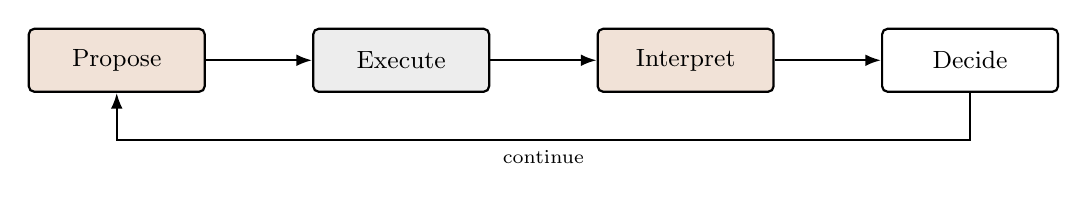
\begin{tikzpicture}[font=\small,node distance=1.35cm,
      b/.style={rectangle,draw,thick,rounded corners=2pt,minimum height=0.8cm,
                text width=2.0cm,align=center},
      llm/.style={b,fill=accent!18},
      det/.style={b,fill=black!7},
      a/.style={-{Latex[length=2mm]},thick}]
      \node[llm] (p)              {Propose};
      \node[det] (e) [right=of p] {Execute};
      \node[llm] (i) [right=of e] {Interpret};
      \node[b]   (d) [right=of i] {Decide};
      \draw[a] (p)--(e); \draw[a] (e)--(i); \draw[a] (i)--(d);
      \draw[a] (d.south) -- ++(0,-0.6) -| node[pos=0.25,below]{\scriptsize continue} (p.south);
    \end{tikzpicture}
  \end{center}
  \begin{itemize}
    \item Same shape as Kubernetes reconciliation
    \item Observe, decide, act, repeat
    \item Shaded steps are model calls
    \item The executor is deterministic
  \end{itemize}
\end{frame}

\begin{frame}{The architecture is three files}
  \begin{columns}[T]
    \begin{column}{0.62\textwidth}
      \begin{itemize}
        \item \texttt{prepare.py} --- data and score
        \item \texttt{train.py} --- model and training
        \item \texttt{program.md} --- the instructions
        \item No scheduler, no driver program
      \end{itemize}
    \end{column}
    \begin{column}{0.36\textwidth}
      \begin{block}{Ownership}
        \small
        nobody edits \texttt{prepare.py}\\
        the agent edits \texttt{train.py}\\
        the human edits \texttt{program.md}
      \end{block}
    \end{column}
  \end{columns}
  \vfill
  \begin{block}{Consequence}
    \texttt{program.md} is not configuration handed to a controller. It is the controller.
  \end{block}
\end{frame}

\begin{frame}{It already works. That is the problem.}
  \begin{itemize}
    \item Shopify Liquid, pull request 2056
    \item \textbf{53\%} faster parse and render
    \item About 120 experiments, 93 commits
    \item Author called it probably overfitted
    \item Never merged
  \end{itemize}
  \vfill
  \begin{alertblock}{The gap}
    Benchmarks report whether a pipeline succeeded. None report which
    instruction was responsible.
  \end{alertblock}
\end{frame}

\begin{frame}{Research questions}
  \begin{block}{RQ1}
    Which components of \texttt{program.md} causally determine which aspects
    of the loop's behaviour, and how large is each effect?
  \end{block}
  \vfill
  \begin{block}{RQ2}
    Do the components act independently of one another?
  \end{block}
  \vfill
  \begin{itemize}
    \item Confounding blocks a direct answer
    \item Reworded files differ in every sentence
  \end{itemize}
\end{frame}

% ======================================================== METHODOLOGY
\begin{frame}{From prose to configuration vector}
  \begin{itemize}
    \item One template, five variable slots
    \item Fixed part byte-identical everywhere
    \item Each slot written at two levels
    \item Nothing else in the file moves
  \end{itemize}
  \vfill
  \begin{block}{A file becomes a vector}
    \centering
    $c=(c_1,\ldots,c_5), \qquad c_i\in\{0,1\}
     \qquad\Longrightarrow\qquad 2^5=32$ files
  \end{block}
\end{frame}

\begin{frame}{Choice of levels: the independent variables}
  \small
  \begin{table}
    \begin{tabular}{@{}clll@{}}
      \toprule
      & \textbf{Component} & \textbf{Level 0} & \textbf{Level 1}\\
      \midrule
      $M$ & Evaluation criterion & success undefined      & 5-fold CV accuracy\\
      $B$ & Search breadth       & one model family       & both families\\
      $S$ & Stopping rule        & fixed 3 experiments    & adaptive, up to 8\\
      $O$ & Reporting style      & terse                  & full sentences\\
      $E$ & Search emphasis      & explore first          & exploit first\\
      \bottomrule
    \end{tabular}
  \end{table}
  \vfill
  \begin{block}{Two controls on the treatment}
    \small
    A second model wrote all ten paragraphs from fixed meta-prompts, then they
    were frozen. The two levels of a slot match to within ten per cent in
    token count.
  \end{block}
\end{frame}

\begin{frame}{Evaluation metrics: the dependent variables}
  \small
  \begin{table}
    \begin{tabular}{@{}ll@{}}
      \toprule
      \textbf{Metric} & \textbf{Definition}\\
      \midrule
      Gain over default   & recommended score minus $a_0(d)$\\
      Wasted trial ratio  & (rejected $+$ duplicate) / attempts\\
      Improvement rate    & share of trials beating the best so far\\
      Cost to best        & executor calls to reach the peak\\
      \bottomrule
    \end{tabular}
  \end{table}
  \vfill
  \begin{block}{Why these, and not judge-based scores}
    \small
    Each is a difference in accuracy, a proportion of proposals, or a count of
    calls, read straight off the structured transcript. No scoring library and
    no judge model enters the measurement, so no metric can drift with the
    instruction being tested.
  \end{block}
\end{frame}

\begin{frame}{Design: run the whole space}
  \begin{block}{Budget}
    \centering
    $N \;=\; \underbrace{2^5}_{\text{configurations}} \times
             \underbrace{D}_{\text{2 tasks}} \times
             \underbrace{R}_{\text{20 replicates}} \;=\; 1{,}280$ runs
  \end{block}
  \vfill
  \begin{itemize}
    \item Configurations built, not collected
    \item Confounding removed by design
    \item Every interaction separately estimable
    \item A fraction would assume RQ2's answer
  \end{itemize}
\end{frame}

\begin{frame}{Controls}
  \begin{columns}[T]
    \begin{column}{0.5\textwidth}
      \begin{itemize}
        \item Pinned model snapshot
        \item One stratified 70/30 split
        \item Same executor and whitelist
        \item Same seed list per cell
      \end{itemize}
    \end{column}
    \begin{column}{0.47\textwidth}
      \begin{alertblock}{Temperature $=0.7$}
        \small
        Not zero, deliberately. Run-to-run variance is the error term. Greedy
        decoding would zero it, and every standard error with it.
      \end{alertblock}
    \end{column}
  \end{columns}
\end{frame}

\begin{frame}{The regression model}
  \begin{block}{Main effects, with the task controlled}
    \centering
    $Y \;=\; \beta_0 \;+\; \sum_{i=1}^{5}\beta_i X_i
       \;+\; \sum_{j=2}^{D}\gamma_j D_j \;+\; \varepsilon$
  \end{block}
  \vspace{0.2cm}
  \begin{itemize}
    \item $Y$: one of four metrics
    \item $X_i$: component $i$, $\pm1$ coded
    \item $D_j$: dataset indicator, the control
    \item $\gamma_j$ absorbs task difficulty
    \item HC3 errors, Benjamini--Hochberg
  \end{itemize}
\end{frame}

% ============================================== RESULTS & LIMITATIONS
\begin{frame}{What moved: the wasted trial ratio}
  \begin{center}
    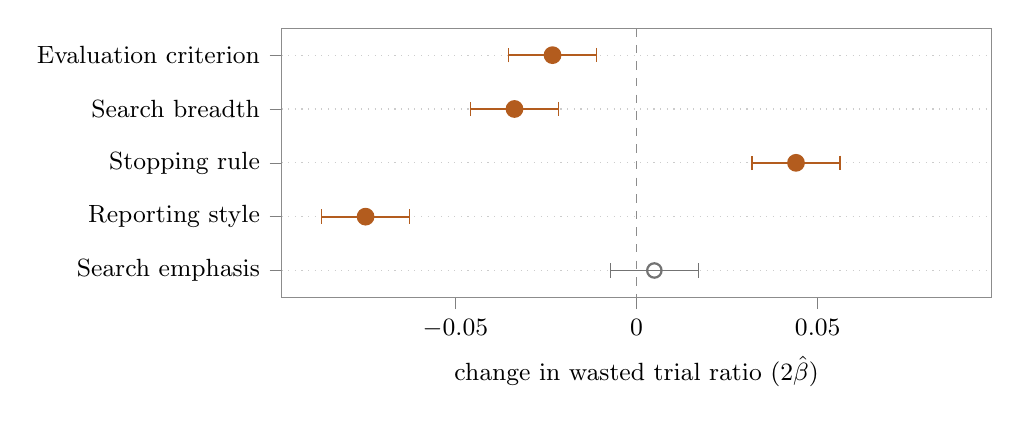
\begin{tikzpicture}
      \begin{axis}[width=10.6cm,height=5.0cm,y dir=reverse,
        ytick={1,2,3,4,5},
        yticklabels={Evaluation criterion,Search breadth,Stopping rule,%
                     Reporting style,Search emphasis},
        ymin=0.5,ymax=5.5,xmin=-0.098,xmax=0.098,
        xlabel={change in wasted trial ratio ($2\hat\beta$)},
        ymajorgrids,major grid style={black!20,dotted},
        axis line style={black!45},tick align=outside,tick pos=left,
        xtick={-0.05,0,0.05},scaled x ticks=false,
        xticklabel style={/pgf/number format/fixed,/pgf/number format/precision=2},
        label style={font=\small},tick label style={font=\small}]
        \addplot[black!45,dashed,forget plot] coordinates {(0,0.5) (0,5.5)};
        \addplot[only marks,mark=*,mark size=2.6pt,accent,very thick,
          error bars/.cd,x dir=both,x explicit,error bar style={accent,thick}]
          coordinates {(-0.02320,1) +- (0.01215,0)
                       (-0.03370,2) +- (0.01215,0)
                       (+0.04400,3) +- (0.01215,0)
                       (-0.07480,4) +- (0.01215,0)};
        \addplot[only marks,mark=o,mark size=2.6pt,black!55,thick,
          error bars/.cd,x dir=both,x explicit,error bar style={black!55}]
          coordinates {(+0.00490,5) +- (0.01215,0)};
      \end{axis}
    \end{tikzpicture}
  \end{center}
  \vspace{-0.2cm}
  {\scriptsize\color{muted}\centering
   filled $=$ survives Benjamini--Hochberg \quad bars $=$ 95\% CI \quad $R^2=0.16$\par}
\end{frame}

\begin{frame}{Results in one slide}
  \begin{itemize}
    \item Reporting style dominates: $-0.075$
    \item Wasted trials $10.6\% \rightarrow 3.1\%$
    \item Stopping rule: only outcome effect
    \item Cost to best: nothing survives
    \item Three of forty interactions significant
  \end{itemize}
  \vfill
  \begin{alertblock}{The task outweighs the instruction}
    \small
    On the improvement rate and the cost to best, the dataset effect is about
    twice the largest component effect, both at $p<10^{-5}$. That is the
    variance $\gamma_j$ removes from the residual.
  \end{alertblock}
\end{frame}

\begin{frame}{Boundary conditions}
  \begin{itemize}
    \item One agent model, one policy
    \item Semantics fixed, phrasing not varied
    \item Two datasets, one contrast
    \item Hyperparameter space, not code
  \end{itemize}
  \vfill
  \begin{block}{Scope of the claim}
    \small
    A proof of concept. It establishes that editing the constraints in
    \texttt{program.md} has a measurable causal influence on the loop's
    behaviour; sizing that influence is left to wider designs.
  \end{block}
\end{frame}

\begin{frame}{Conclusion}
  \begin{itemize}
    \item Instructions govern process, not outcome
    \item Verbose reporting: two thirds less waste
    \item Components act independently
    \item Method transfers to any sliced prompt
  \end{itemize}
  \vfill
  \begin{block}{Why outcome barely moved}
    \small
    Untuned defaults already reach $a_0=0.960$ on both tasks and only $40\%$
    of runs improve on that. The ceiling binds, not the loop.
  \end{block}
  \vfill
  \centering\small Thank you. Questions welcome.
\end{frame}

\end{document}
